\documentclass{article}
\usepackage{graphicx}
\usepackage[margin=2.5cm]{geometry}
\usepackage{listings}
\lstset{language=Python}
\usepackage{hyperref}
\usepackage{minted}
\usepackage{amsmath}
\usepackage{tikz, pgfplots}
\usetikzlibrary{positioning}
\usepackage{parskip}
\usepackage{adjustbox}
\usepackage{amssymb}
\usepackage{caption}

\begin{document}

\title{
    {ESW Project: Obstacle avoidance ground robot}\\
    {Team 5}\\
    {\large International Institute of Information Technology, Hyderabad}\\
    \author{Abhinav Raundhal, Yash Shinde, Samyak Mishra, Vinit Mehta}
    \vspace{1cm}
    
\includegraphics[width=3cm]{IIITH.png}
}
\date{}

\maketitle

\section{Control Sequence}
    \begin{center}
    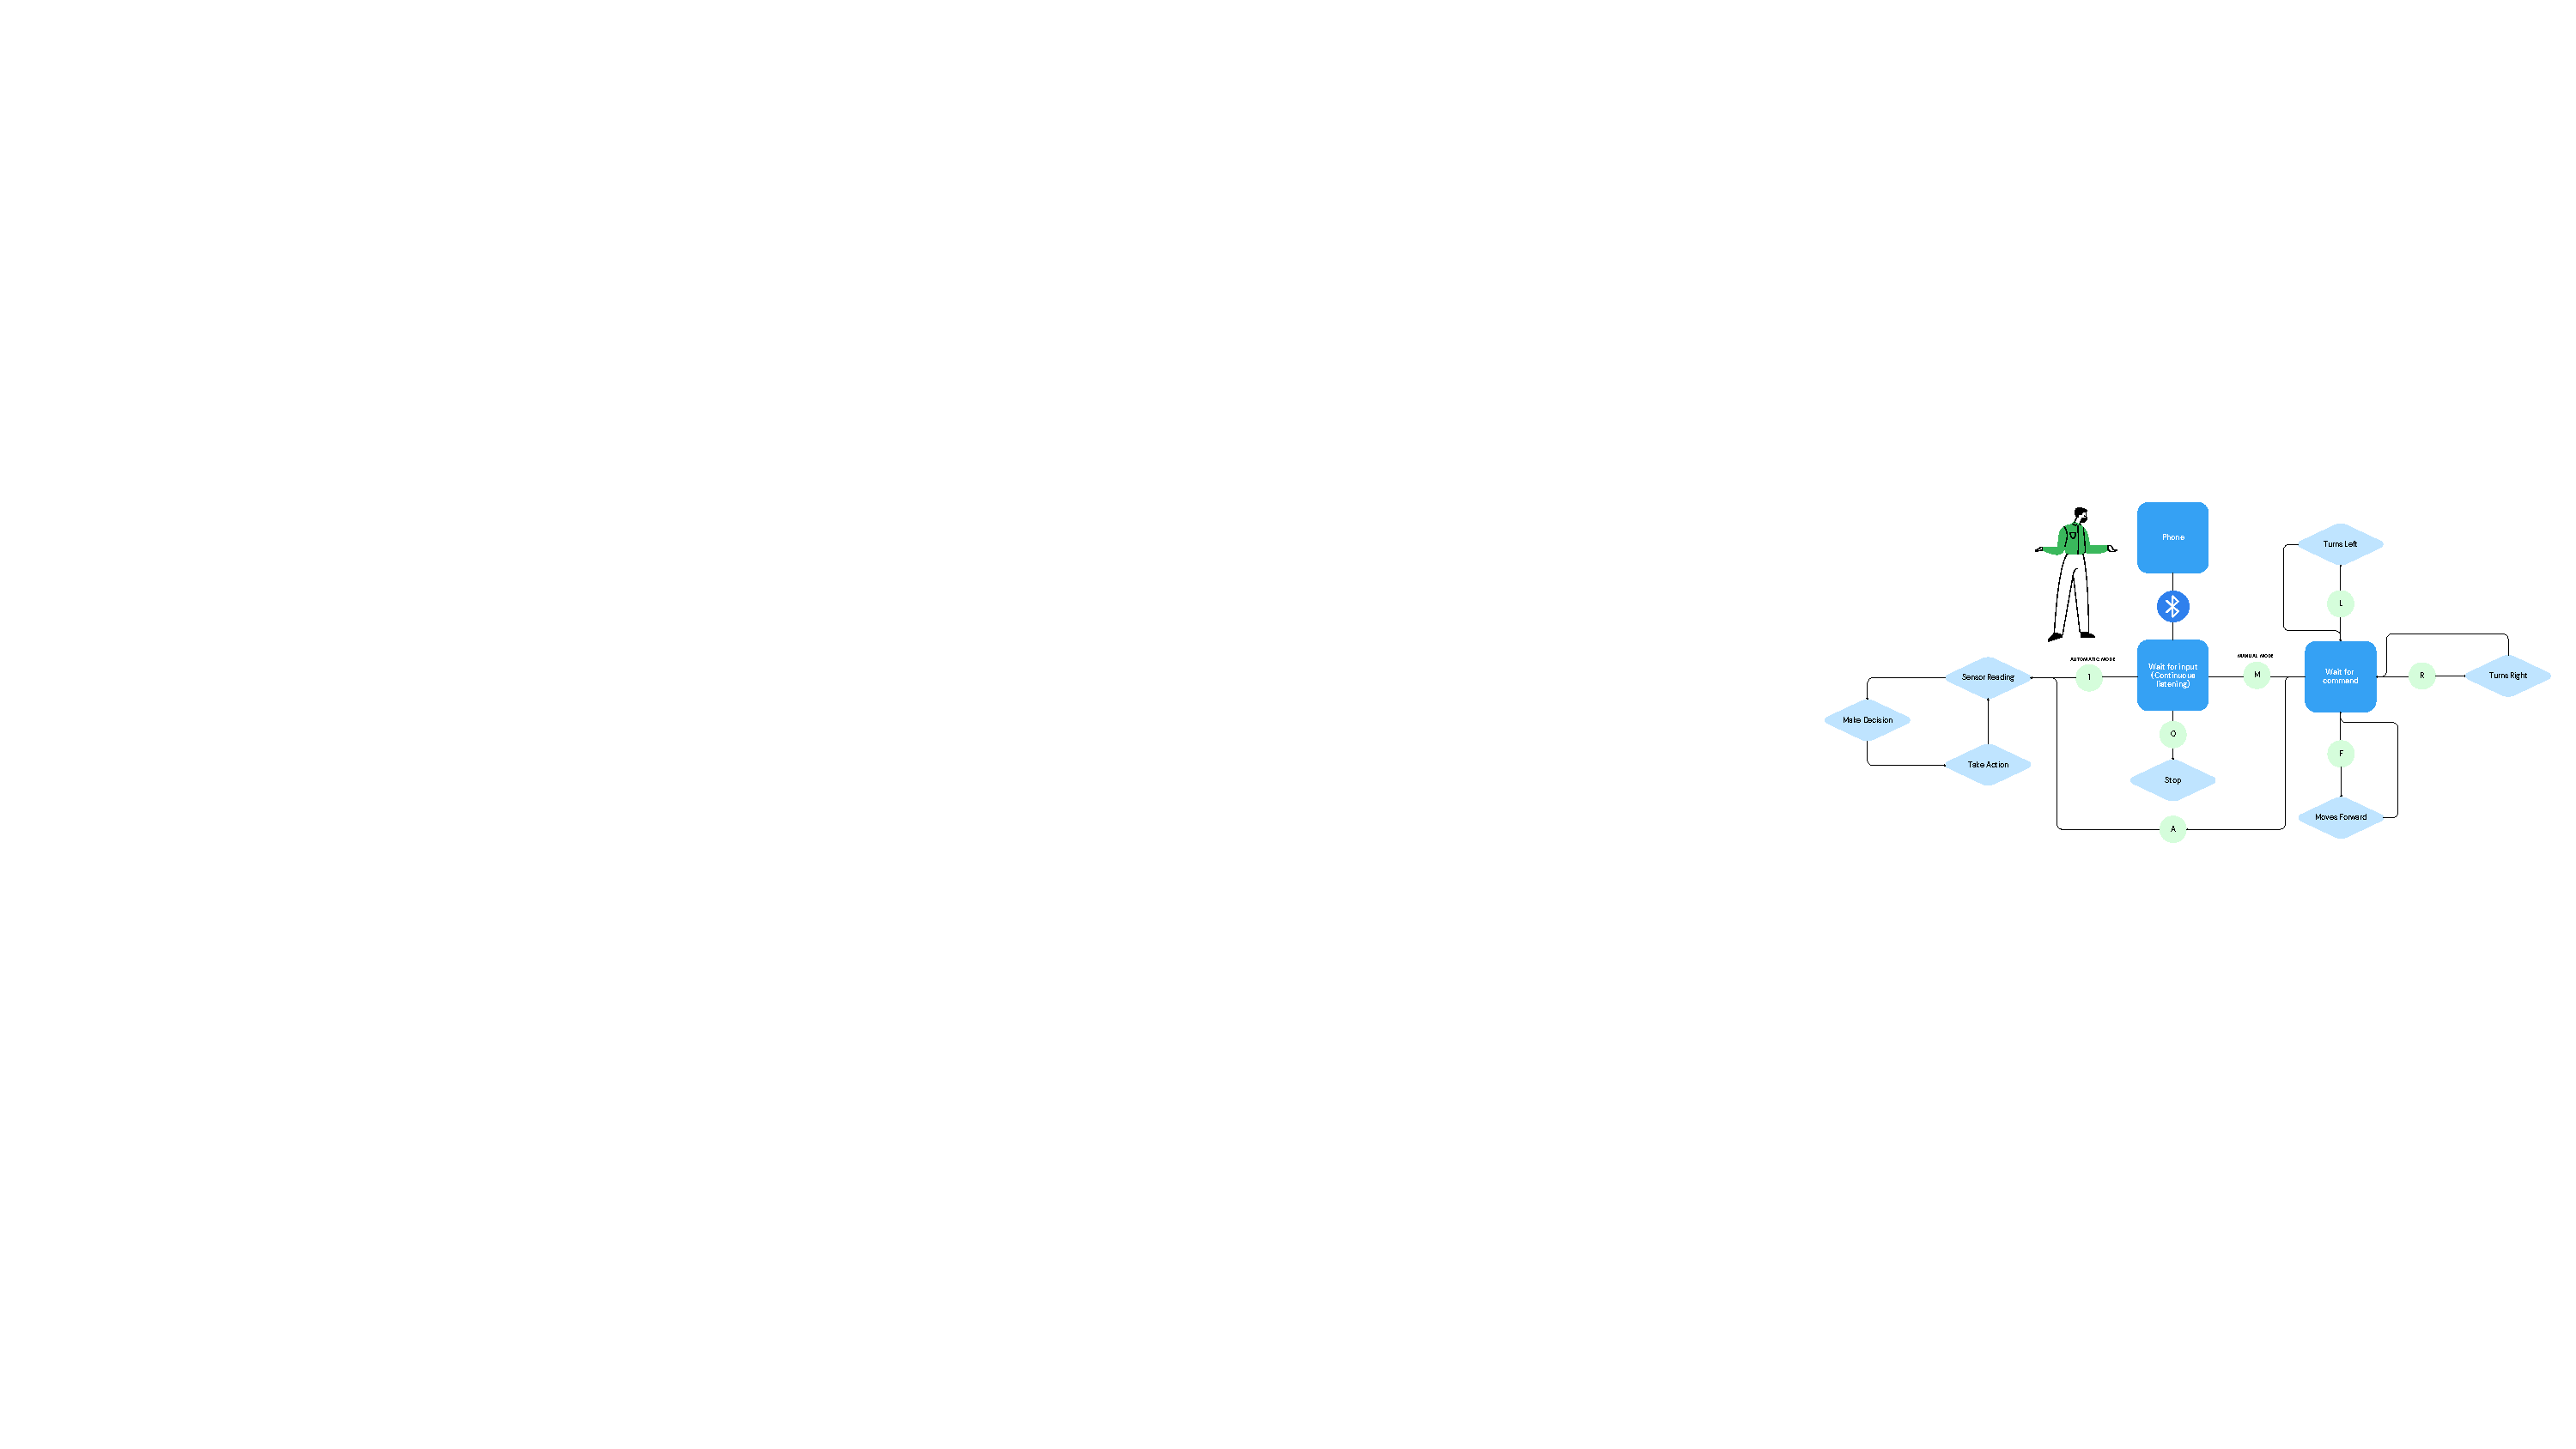
\includegraphics[width=15cm]{flowchart.pdf}
    \end{center}
    The communication between the phone and the ESP begins by establishing a Bluetooth connection. Once connected, the ESP establishes a WiFi connection. The ESP module then enters a standby state, awaiting input from the paired phone.

    Upon receiving the command '1', the ESP transitions into automatic mode. In this mode, it initiates a sequence: first, it reads sensor data to gather information about its environment. Based on these readings, the microcontroller intelligently determines the appropriate actions for the robot. The motors are then directed accordingly to navigate the robot through its environment. This process repeats indefinitely until the command '0' is received, signaling the robot to stop.

    Alternatively, if the command 'm' is received, the robot switches to manual mode. In manual mode, the robot awaits user commands. The commands include 'r' for turning right, 'l' for turning left, 'f' for continuous forward movement until a '0' is received, or until an obstacle is encountered, prompting an automatic halt. If the command 'a' is given, the robot seamlessly shifts back to automatic mode.

\section{Information flow}
    \begin{center}
    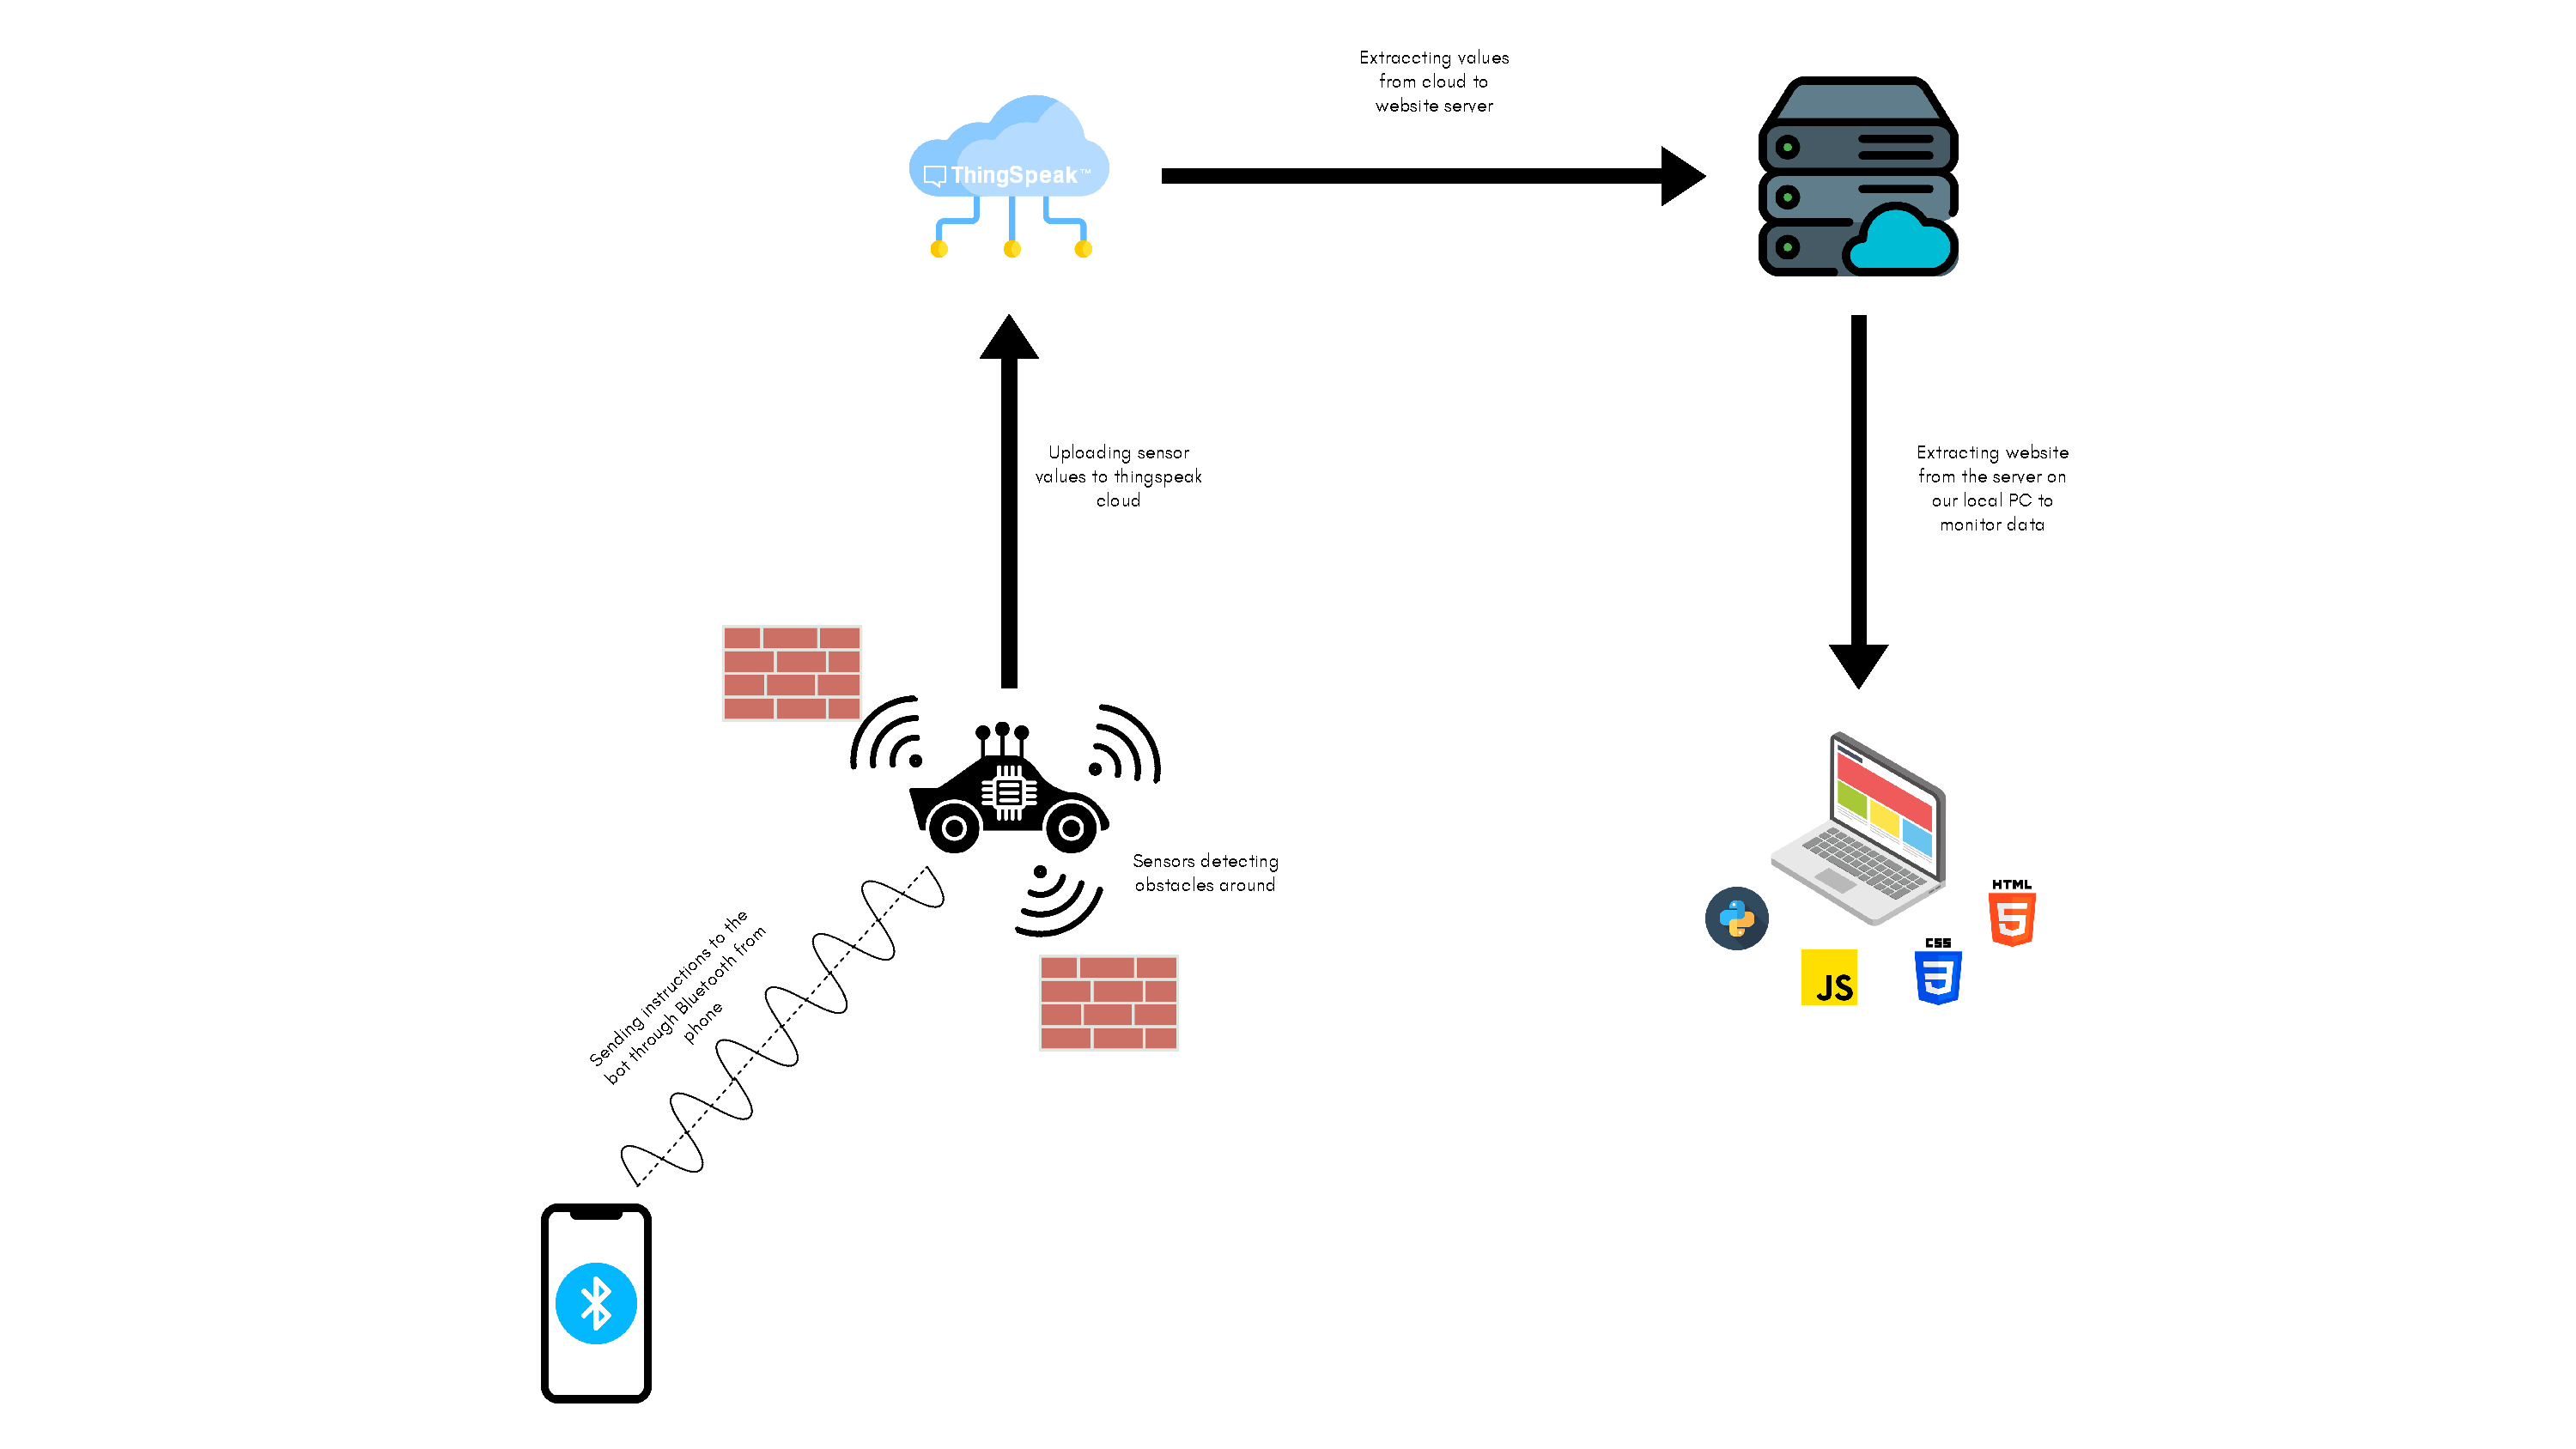
\includegraphics[width=15cm]{working.pdf}
    \end{center}
    
    The initial step involves establishing a Bluetooth connection between the mobile device and the robot. Once connected, the robot engages in autonomous navigation, skillfully maneuvering through its environment while intelligently avoiding obstacles. Concurrently, it periodically uploads data to the ThingSpeak cloud platform.

    The data uploaded to ThingSpeak is subsequently extracted and transmitted to our server, where our website is hosted. Users can conveniently access this data through the website's URL, providing a seamless and user-friendly interface. The information is presented in the form of visually informative graphs, enabling users to observe and analyze the robot's journey and interactions with its surroundings from the convenience of their local machines.

    In addition to its autonomous navigation and obstacle avoidance capabilities, the robot's interaction with the ThingSpeak cloud platform serves as a pivotal aspect of its functionality. As the robot traverses its environment, it not only prioritizes real-time decision-making but also diligently collects data related to its surroundings.

    The data, consisting of crucial metrics and sensor readings, is regularly transmitted to the ThingSpeak cloud platform. This cloud-based repository acts as a dynamic hub for storing and managing the robot's operational data. The use of ThingSpeak facilitates a seamless integration of Internet of Things (IoT) principles into the robot's operational framework.

\section{Circuit Diagram}
    \begin{center}
    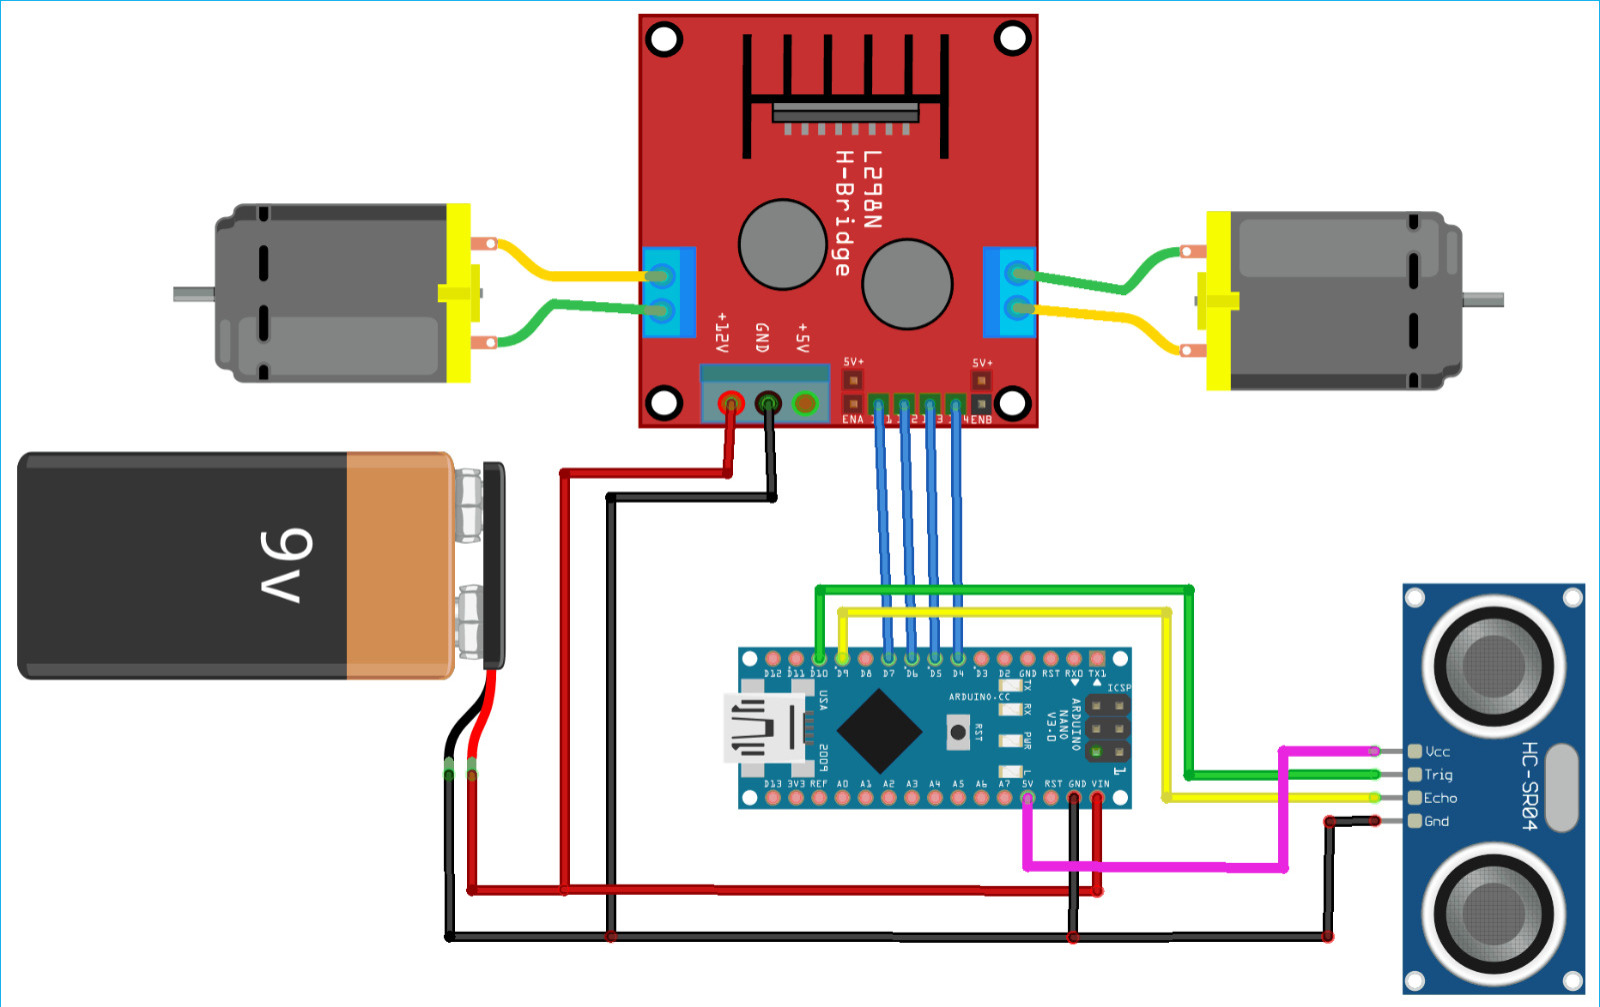
\includegraphics[width=15cm]{circuit-diagram.jpeg}
    \end{center}
    The seamless coordination of the robotic system involves a precise orchestration of components, each contributing to the robot's intelligent navigation. At the core of this functionality is the microcontroller, which orchestrates a sophisticated dance between the sensory input and motor control.

    The microcontroller, as the brain of the system, commands five ultrasonic sensors strategically placed to capture the robot's surroundings comprehensively. Once activated, these sensors promptly gather readings, providing a real-time snapshot of the distances to nearby objects. This wealth of data becomes the foundation for the subsequent decision-making process.

    In the heart of the microcontroller resides an algorithm designed to process the sensor readings and make informed decisions. The algorithm takes into account the spatial information gleaned from the ultrasonic sensors, assessing the environment for obstacles and determining the optimal path forward. The decisions made by the algorithm serve as a set of instructions guiding the robot through its surroundings.

    Upon reaching a decision, the microcontroller seamlessly communicates with the motor driver. This interaction triggers the motor driver to initiate precise maneuvers by controlling the motors. The motor controller, acting as the intermediary, redirects the high-voltage current from the external battery source to the motors. This redirection ensures that the motors rotate at the specified speed, facilitating accurate turns and movements in alignment with the algorithm's directives.

    The iterative nature of this process forms a continuous loop, creating a responsive and adaptive system. As the ultrasonic sensors continuously gather data, the microcontroller, algorithm, and motor control work in tandem to navigate the robot through its environment. This dynamic feedback loop allows the robot to adapt swiftly to changing conditions, demonstrating an intelligent and efficient approach to autonomous navigation.

    In summary, the microcontroller serves as the orchestrator, seamlessly integrating sensor input, algorithmic decision-making, and motor control. This collaborative interplay ensures the robot's ability to navigate and respond intelligently to its surroundings, making it a versatile and effective autonomous system.

\section{Image gallery}

\vspace{1cm}

\begin{center}

\begin{minipage}{0.3\textwidth}
    \centering
    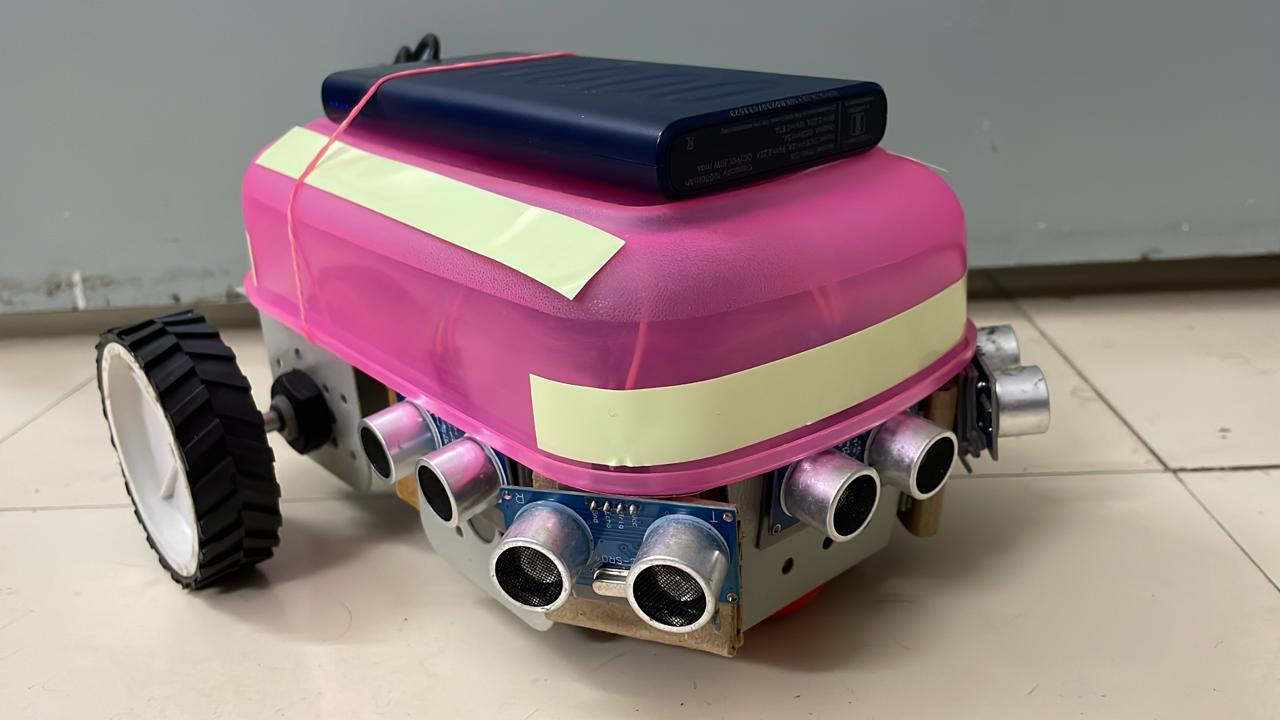
\includegraphics[width=\linewidth]{bot.jpeg}
    Our bot
\end{minipage}
\hfill
\begin{minipage}{0.3\textwidth}
    \centering
    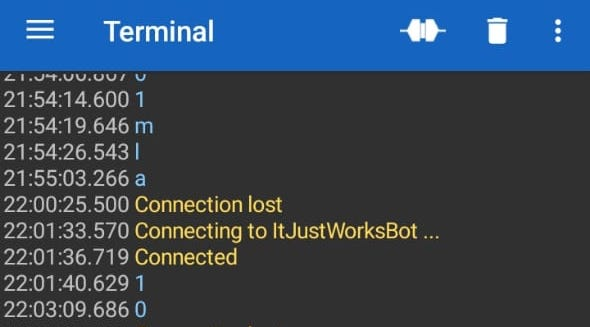
\includegraphics[width=\linewidth]{bluetooth-phone.jpeg}
    Sending instructions
\end{minipage}
\hfill
\begin{minipage}{0.3\textwidth}
    \centering
    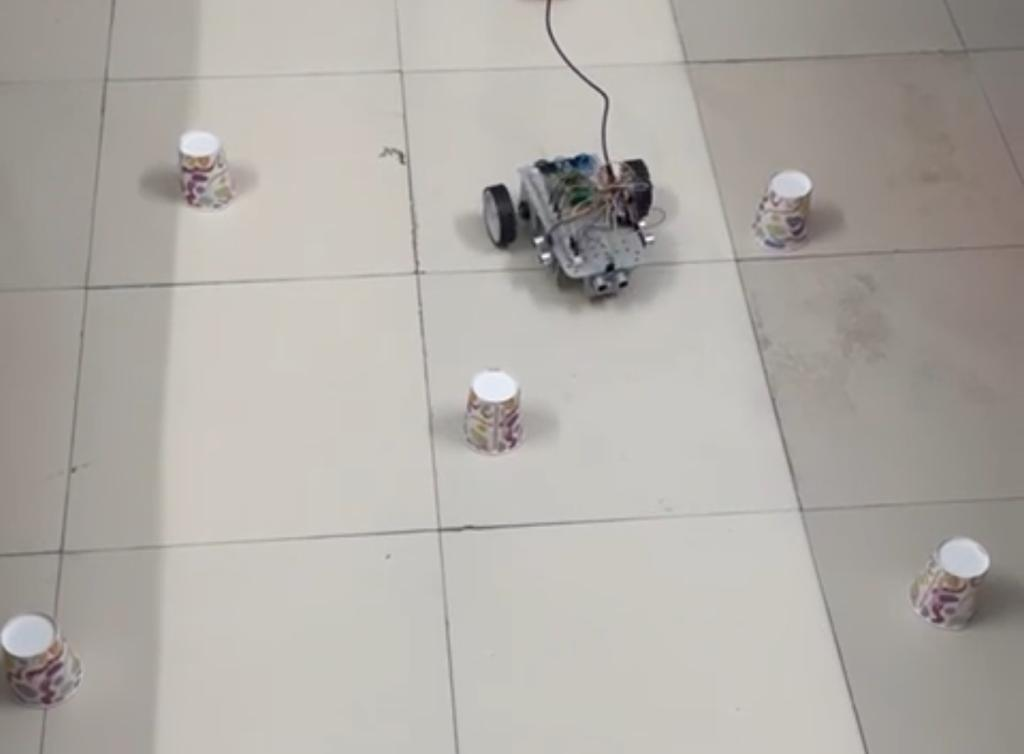
\includegraphics[width=\linewidth]{bot-moving.jpeg}
    Bot navigating
    \vspace{0.5cm}
\end{minipage}
\hfill
\begin{minipage}{0.4\textwidth}
    \centering
    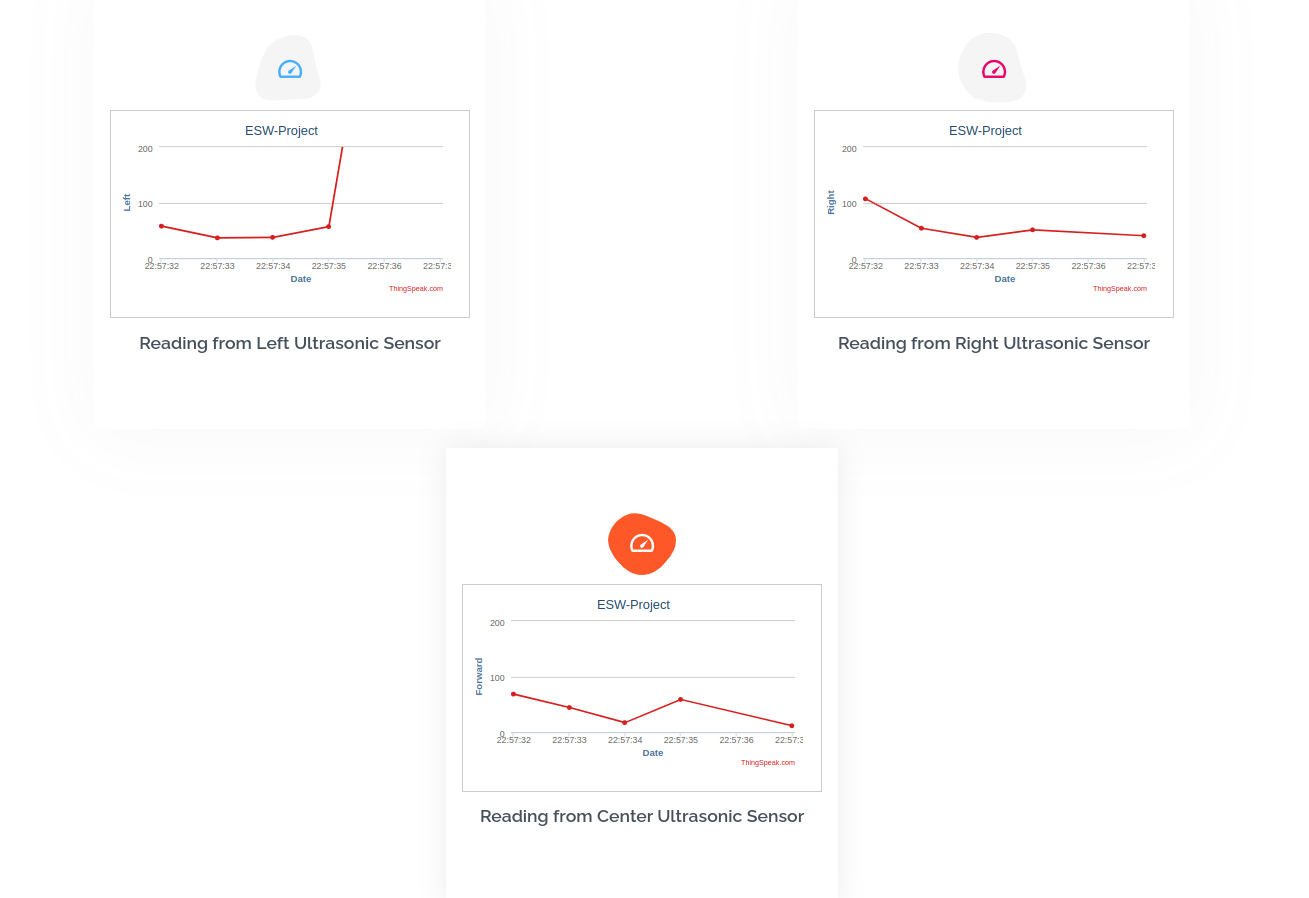
\includegraphics[width=\linewidth]{website-graph.png}
    Graph of sensor readings
\end{minipage}
\hfill
\begin{minipage}{0.5\textwidth}
    \centering
    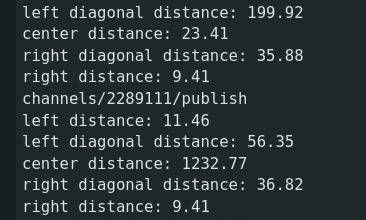
\includegraphics[width=\linewidth]{data-publish.jpeg}
    Publishing data
    \vspace{0.5cm}
\end{minipage}
\hfill
\begin{minipage}{1.0\textwidth}
    \centering
    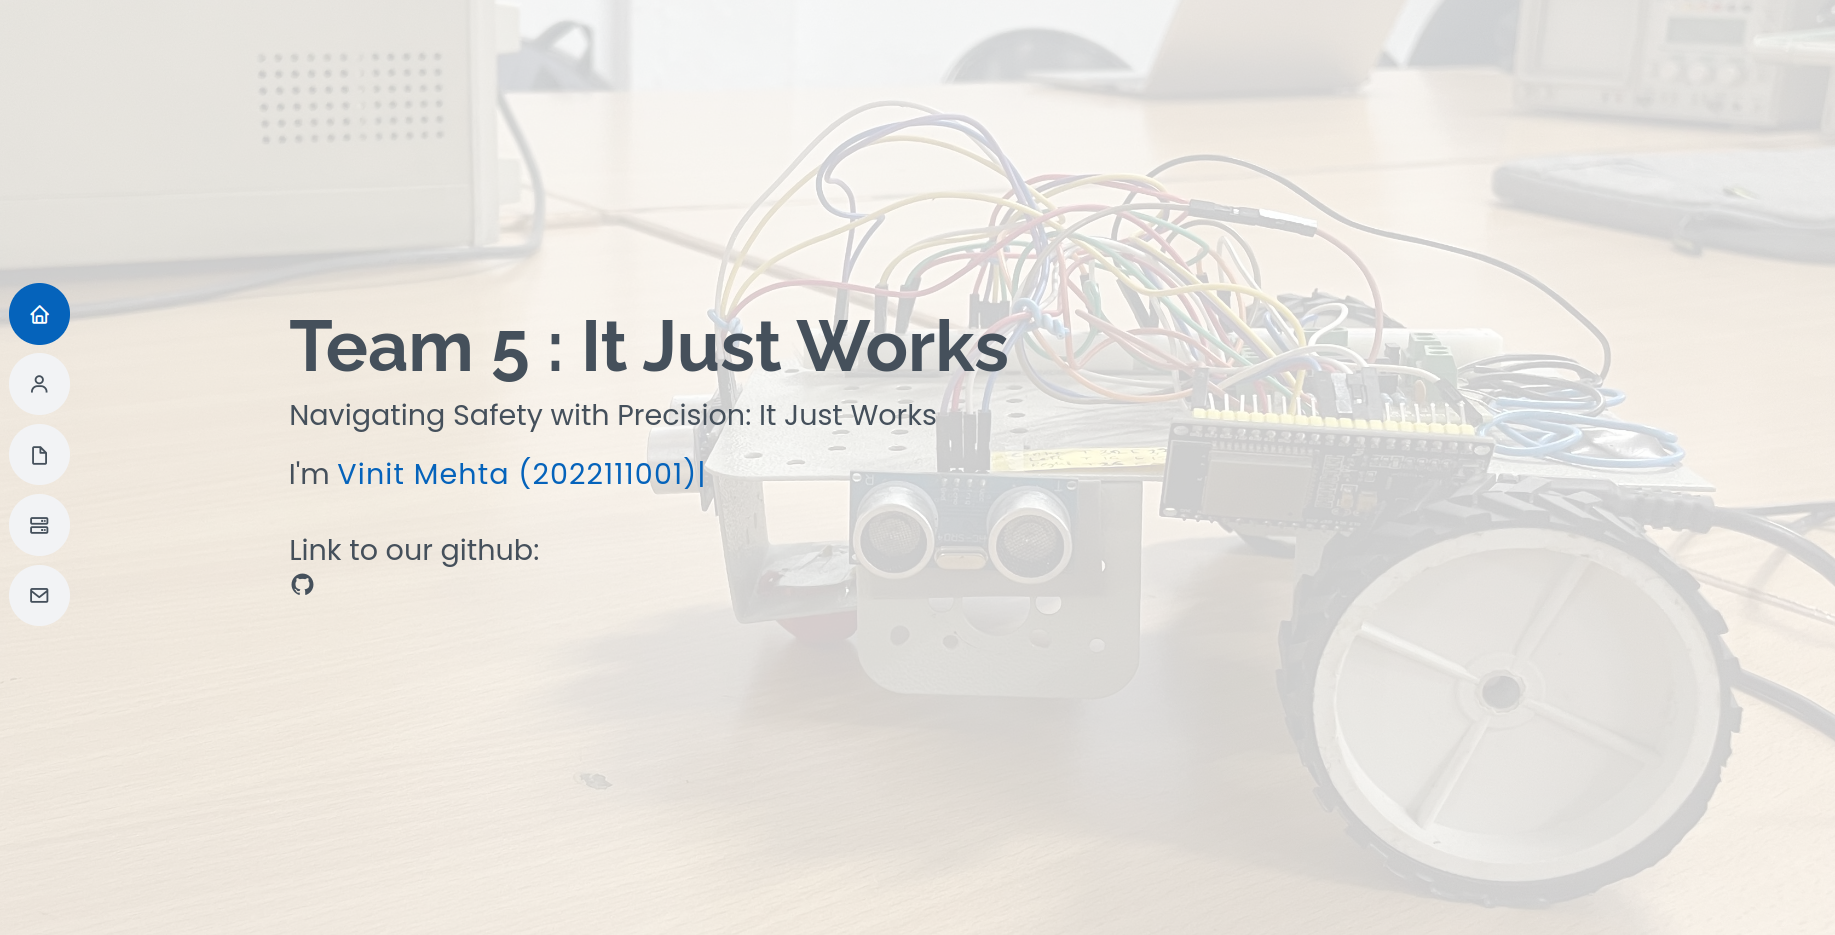
\includegraphics[width=\linewidth]{website-front.png}
    Website
\end{minipage}

\end{center}

\section{Appendix}
Click \href{https://github.com/Vinit2244/ESW-Project-It-Just-Works}{here} to go to our github.


\end{document}
